\documentclass[conference,10pt]{IEEEtran}
%\documentclass{article}
\IEEEoverridecommandlockouts
%\usepackage[T1]{fontenc}
%\usepackage[utf8]{inputenc}
%\usepackage[style=ieee]{biblatex}
%\usepackage[numbers]{natbib}

%\usepackage{algorithm2e}
\usepackage{algorithm}
\usepackage[noend]{algpseudocode}
\newcommand{\vars}{\texttt}
\newcommand{\func}{\textrm}
\let\oldReturn\Return
\renewcommand{\Return}{\State\oldReturn}
\newcommand*\Let[2]{\State #1 $\gets$ #2}
\algrenewcommand\alglinenumber[1]{
  {\sf\footnotesize\addfontfeatures{Colour=888888,Numbers=Monospaced}#1}
}
\algrenewcommand\algorithmicrequire{\textbf{Precondition:}}
\algrenewcommand\algorithmicensure{\textbf{Postcondition:}}

\usepackage{comment}
\usepackage{xurl}
\usepackage{hyperref}
\usepackage{graphicx}
\usepackage[table,xcdraw]{xcolor}
\usepackage[caption=false]{subfig}
\usepackage{minted}
\usepackage{multirow}
% Configure hyperlinks
%\hypersetup{
%  colorlinks=true,
%  linkcolor=blue,
%  filecolor=magenta,
%  urlcolor=blue,
%}
% Custom colors
%\definecolor{lightergray}{gray}{0.9}
% Global configs
%\graphicspath{{./out/}}
%\addbibresource{src/bibliography.bib}

\usepackage{caption}
\captionsetup{font=footnotesize}

\usepackage{tabularx}
\usepackage{mathtools}
\usepackage{xparse}
\usepackage[parfill]{parskip}
\usepackage{csquotes}
\usepackage{siunitx}
\usepackage{textcomp}
\usepackage{tikz}
% \usepackage{listings}
% \usepackage{lipsum}
% \usepackage{blindtext}
%\usepackage{unicode-math}

\newcommand{\ignore}[1] {}
\pagenumbering{arabic}
\pagestyle{plain}

% Message
\newcommand{\kk}[1]{{{\color{red} #1}}}
\newcommand{\ds}[1]{{{\color{blue} #1}}}
\newcommand{\su}[1]{{{\color{green} #1}}}

% Shortcuts
% \newcommand{\hyprCPU}{HyPR (Pure CPU)}
% \newcommand{\hyprGPU}{HyPR (Pure GPU)}
% \newcommand{\sticdPR}{Algorithm SticdPR}
\newcommand{\monolithicPR}{Algorithm \textsc{DynamicMonolithicPR}}
\newcommand{\levelwisePR}{Algorithm \textsc{DynamicLevelwisePR}}
\newcommand{\gscc}{G_{\mathrm{SCC}}}
% \NewDocumentCommand{\codeword}{v}{\texttt{\textcolor{blue}{#1}}}

\newcommand{\X}{$\times$}
\newcommand{\x}{$\times$}




\title{Dynamic Batch Parallel Algorithms for Updating PageRank}
\author{
  \IEEEauthorblockN{
    Subhajit Sahu\IEEEauthorrefmark{2}$^*$ \thanks{$^*$The work of this author is partially supported by a grant from the Department of Science and Technology (DST), India, under the National Supercomputing Mission (NSM) R\&D in Exascale initiative vide Ref. No: DST/NSM/R\&D\_Exascale/2021/16.},
    Kishore Kothapalli\IEEEauthorrefmark{2}$^*$ and
    Dip Sankar Banerjee\IEEEauthorrefmark{3}}
  \IEEEauthorblockA{
    \IEEEauthorrefmark{2}International Institute of Information Technology Hyderabad, India.}
    \IEEEauthorblockA{\IEEEauthorrefmark{3} Indian Institute of Technology Jodhpur, India.\\
      \{subhajit.sahu@research.,kkishore@\}iiit.ac.in, dipsankarb@iitj.ac.in}
    }
\date{}




\begin{document}
\maketitle
\begin{abstract}
The design and implementation of parallel algorithms for dynamic graph problems is attracting significant research attention in the recent years, driven by numerous applications to social network analysis, neuroscience, and protein interaction networks. One such problem is the computation of PageRank values of vertices in a directed graph.
This paper presents two new parallel algorithms for recomputing the PageRank values of vertices in a dynamic graph. Our techniques require the recomputation of the PageRank of only the vertices affected by the insertion/deletion of a batch of edges. We conduct detailed experimental studies of our algorithm on a set of 11 real-world graphs. Our results on Intel Xeon Silver 4116 CPU and NVIDIA Tesla V100 PCIe 16GB GPU indicate that our algorithms outperform static and dynamic update algorithms by 6.1\x and 8.6\x on the CPU, and by 9.8\x and 9.3\x on the GPU respectively. We also compare the performance of the algorithms in batched mode to cumulative single-edge updates.
\end{abstract}

\section{Introduction}
Graphs offer an effective way to capture meaningful relationships between data. Due to the growing size of our data, today there is tremendous interest in parallel algorithms for a variety of graph problems. One such graph problem is computing the PageRank of vertices in a graph, a measure that is based on each vertex's relative importance in the graph. It is a popular measure with applications such as ranking the websites \cite{page}, the scientific impact of researchers \cite{zomaya}, in the analysis of protein networks \cite{protein}, and in applications of neuroscience \cite{neuro}. It is therefore not surprising that there is recent interest in computing the PageRank values of vertices in a graph on shared memory architectures \cite{pr-sticd16,hipc17} and GPUs \cite{hipc19}. These approaches use a variety of solution approaches, viz., iterative, random walk, and matrix multiplication.

A limitation of the algorithms mentioned above for obtaining PageRank values on graphs is that the graph is static. However, networks from domains of applications to PageRank, such as protein networks, the web graph, collaboration networks, evolve with the insertion/deletion of edges/vertices. For the above algorithms to work on such evolving graphs, the only recourse is a full recomputation, which can be expensive given the large size of the graphs of interest.

A solution to this problem is to use dynamic graph algorithms that efficiently update a graph analytic upon the insertion/deletion of edges/vertices. Several authors have investigated dynamic algorithms for graph problems in the standard sequential computing model. These led to dynamic algorithms for fundamental problems on graphs such as connectivity, bi-connectivity, shortest paths, transitive closure, bipartite testing, and the like (see for instance \cite{eppstein}, and the references therein). On the other hand, parallel algorithms in this setting are relatively new. Some of the recent examples in the parallel setting include the work of Jamour et al. \cite{jamour}, Regunta et al. \cite{cent-shukla20}, and Mc Coll et al. \cite{cc-mccoll13}.

Many sequential dynamic graph algorithms follow the nomenclature of being incremental, decremental, or fully dynamic. An incremental algorithm can handle a {\em single} edge/vertex insertion (deletion for decremental). On the other hand, a fully dynamic algorithm can handle any single edge/vertex update (insertion or deletion). A parallel dynamic graph algorithm can, in addition, leverage parallelism owing to a batch of updates instead of a single edge/vertex update. Compared to a single update, a batch update also offers scope for reducing the overall work. We refer to such algorithms as {\em batch dynamic parallel graph algorithms}. 

Given the huge number of applications of PageRank, it is pertinent to design and engineer batch dynamic parallel algorithms that update the PageRank values of vertices without a full re-computation. In a recent work~\cite{hipc19} on this problem, Giri et al. propose the HyPR parallel algorithm which can update the ranks of an existing graph using a batch of edges on a heterogeneous computing platform consisting of a CPU and a GPU. The algorithm from \cite{hipc19} operates via updating the PageRank of all the affected vertices. However, identifying affected vertices from an inherently irregular graph leads to unbalanced parallel work which can be sub-optimal.

In this paper, we arrive at fully dynamic batch parallel algorithms for updating the PageRank values of vertices in a graph. Our algorithms work on both multicore CPUs and accelerators such as GPUs. Our algorithms identify affected vertices in sets of the strongly connected components (SCCs) of the underlying graph thereby improving on the work of \cite{hipc19}.




\subsection{Our Results}

Below is a summary of our results. We propose two dynamic parallel PageRank algorithms: \monolithicPR{} ({\bf Algorithm \ref{alg:monolithic}}), and \levelwisePR{} ({\bf Algorithm \ref{alg:levelwise}}). Both algorithms are based on the idea that they update the PageRank values of only the {\em affected} vertices in the SCCs of the graph under the insertion/deletion of a batch of edges.

We conduct detailed experimental studies on a collection of 11 real-world graphs (of four different classes) on an Intel multicore CPU, and an NVIDIA GPU. We observe the following:
\begin{itemize}
\item On the CPU, we observe a mean speedup of {4.2\X/5.8\X} for \monolithicPR{} and \levelwisePR{} respectively with respect to a pure CPU implementation of HyPR \cite{hipc19}, a state-of-the-art dynamic PageRank algorithm that only recomputes ranks of affected vertices in the graph. We observe a mean speedup of {6.1\X/8.6\X} with respect to the STIC-D algorithm \cite{pr-sticd16}, a static algorithm that recomputes the PageRank of all vertices in the graph. The above numbers the average of results obtained on batch sizes ranging from 500, 1000, 2000, 5000, and 10000 edges with an equal mix of insertions and deletions.
\item On the GPU, we observe a mean speedup of {1.9\X/1.8\X} for \monolithicPR{} and \levelwisePR{} respectively with respect to a pure GPU implementation of HyPR. We observe a mean speedup of {9.8\X/9.3\X} with respect to naive dynamic version of nvGraph PageRank \cite{pr-nvgraph}, a dynamic algorithm that computes the ranks of all vertices in the graph from the previous ranks of vertices. These observations are made on a similar set of batches.
\item In addition, we show that both our algorithms running on a batch of updates offer an advantage of {4066\X/2998\X} for \monolithicPR{} and \levelwisePR{} respectively on the CPU, and {1712\X/2324\X} on the GPU, over cumulative single-edge update version of the same algorithms on a batch size of 5000 edges with an equal mix of insertions and deletions.
\end{itemize}




\subsection{Related Work}

Techniques to improve the practical performance of algorithms for PageRank are a topic of recent research. Some of these, viz. \cite{pr-arasu02,pr-block03,pr-duong12} are directed only towards web graphs and may not translate to other real-world graphs. Broder et al. \cite{broder00} characterize the structure of web graphs as having a bow-tie nature with a large strongly connected component (SCC), and having a large number of incoming and outgoing edges. Arasu et al. \cite{pr-arasu02} use this characterization to represent PageRank as a solution to a set of independent matrix equations on a block upper triangular matrix. Kamvar et al. \cite{pr-block03} extend the characterization from Broder et al. \cite{broder00} to partition the input graph into blocks. Each block corresponds to a set of vertices in the same physical domain, and hence are naturally related. They compute a PageRank local to each block, called the {\em local} PageRank, and a PageRank for the blocks called as {\em BlockRank}. The final PageRank of vertices is a function of these two ranks. The final ranks thus computed by Kamvar et al. \cite{pr-block03} are approximate ranks and can differ from the PageRank values computed without using the block structure of the graph.

Other approximation based approaches include the work of SiteRank by Wu and Aberer \cite{wu}, the U-Model work of Broder et al. \cite{broder}, the ServerRank work of Wang et al. \cite{wang}, and the HostRank/DirRank work of Eiron et al. \cite{eiron}. Kohlschutter et al. \cite{kohlschutter} extend the results of Kamvar et al. \cite{pr-block03} to obtain exact PageRanks. 

One limitation of these works \cite{pr-block03,eiron,kohlschutter,wang,wu} is that their algorithms are tailored towards web graphs and may not work well for general-purpose graphs. As the PageRank measure finds applications in other domains, generic techniques find prominence. Garg et al. \cite{pr-sticd16} propose a multicore algorithm for obtaining PageRank values based on level-wise arrangement of the SCCs of the graph. This algorithm also introduces additional optimizations such as eliminating identical vertices, chain vertices, and vertices with converged ranks. Further improvements to this paper are reported by Panyala et al. \cite{hipc17}.

Parallel computation of PageRank on emerging architectures such as GPUs has been studied by Duong et al. \cite{pr-duong12}. The work does not introduce any algorithmic optimizations in the computation of PageRank. On the other hand, we believe that our algorithmic techniques will also apply to other architectures.

Expressing the PageRank computation as a Markov chain and solving for the steady-state transition probabilities of the underlying Markov chain is a mechanism used by many authors. Pandurangan et al. \cite{pr-sarma13} study such an approach in the distributed setting.

Importantly, all these consider only the static setting where the underlying graph does not change over time. Ramalingam \cite{incr-ramalingam96} argues for measuring the work done by a dynamic graph algorithm as a function of the change in the input and output, calling it as {\em bounded incremental computation}. The book presents bounded incremental algorithms in the sequential model for graph problems like shortest paths, circuit value annotation, and reducible flow graphs.  

Parallel dynamic graph algorithms on modern architectures are presented by Giri et al. \cite{hipc19} for PageRank, Regunta et al. \cite{cent-shukla20}, Haryan et al. \cite{cent-shukla20} for betweenness- and closeness-centrality, Bhowmick et al. \cite{sssp-khanda22} for shortest paths, and Bader et al. \cite{cc-mccoll13} for connectivity. The HyPR algorithm proposed by Giri et al.~\cite{hipc19} proposed a CPU+GPU hybrid implementation strategy for computing the PageRank scores on batches of heterogeneous updates. The batches contained a mix of both insert and delete operations and the data parallel operations were centered around the affected vertices in the graph. This may lead to limited utilization of the GPU since the number of affected vertices can vary widely depending upon the structure of the graph. The solution proposed in this paper is centered around the identification of the affected components of the graph rather than the vertices which leads to a extraction of higher amounts of parallelism at different levels of granularity.




% Monolithic Dynamic PageRank on an insert/delete batch of 5000 edges performs xx times faster than the nvGraph library implementation of a  static algorithm that recomputes the PageRank of all vertices in the graph. 
%Parallel algorithms often have to also contend with challenges from the architectural environment they are working on. It is common to encounter parallel algorithms that are efficient on one parallel architecture and inefficient on a different architecture. Hence, it is required that algorithm designers consider also the underlying architectural environment and arrive at algorithms that work well on a given architecture. In the present case too, we notice that our algorithm on multicore CPUs ({\bf cf.} Algorithm [monolithic] is not suitable for \emph{distributed CPU/GPUs}. We therefore have two separate algorithms: one for the GPU and one for the CPU. 


%\kk{REVISE *** Citations from ICDCN 2016 paper}


%\su{Sir we can also discuss about PageRank on large graphs, as in this paper "Scaling PageRank to 100 Billion Pages" where he discusses about the process of communicating ranks between partitions of the graph. With levelwise method we can avoid per-iteration communication (as long as each SCC fits on a PC).}
%\su{We could also discuss on the various variants of PageRank, like topic-sensitive PageRank.}


\section{Preliminaries}
\subsection{Static PageRank}

PageRank~\cite{page} is computed on a graph $G(V, E, w)$ where $V$ ($n = |V|$) is the set of vertices representing the web pages, $E$ ($m = |E|$) is the set of edges representing the hyperlinks, and $w$ is the set of edge weights which represent the \emph{contribution} of a vertex to the vertex it connects with via an edge. Using the random-surfer model, which accounts for any random internet user to land at a particular page, the rank of a vertex $v$ is given as:

\begin{equation}
\label{eq:pr1}
    pr_v = \sum_{u \in in_v} c_{u \rightarrow v} + \frac{1 - d}{n}
\end{equation}

In Equation~\ref{eq:pr1}, $d$ is the \emph{damping factor} (taken as $0.15$ conventionally), which represents the probability of a random surfer jumping to a random page on the internet, instead of following one of the links on the given page. The function $c_{u \rightarrow v}$ is the contribution of PageRank score from a page $u$ pointing to the given page $v$. Its magnitude is proportional to the PageRank score of the pointing page ($u$) $pr_u$, and is inversely proportional to the degree of the pointing page ($u$) $outdeg_u$, such that the total value of contributions from $u$ never exceeds its own rank $pr_u$. It is expressed as:

\begin{equation}
\label{eq:pr2}
c_{u \rightarrow v} = (1 - d) \times  \frac{pr_u}{outdeg_u}
\end{equation}

For static PageRank computation (from scratch) we will refer to baseline algorithm as discussed in Garg et al.~\cite{pr-sticd16}. At the beginning they consider PageRank score to be $d/n$ where $d$ is damping factor and $n$ is number of vertices. Furthermore, they compute new PageRank of every vertex considering the contribution provided by its incoming neighbours.

In Equation~\ref{eq:pr2}, we observe that PageRank computations can happen via cyclic contributions of two vertices on each other. Thus, PageRank values are iteratively computed for all vertices until they converge. This signifies that there are small updates to the scores after a particular iteration. This style of computing PageRank scores is popularly done through \emph{power iterations}~\cite{page}. Power iterations arises from the idea of modeling the computations of the PageRank scores as a Markov chain that reaches a steady state when starting from an initial distribution. Here, the initial scores compose the starting states of every vertex which then go through several transitions to reach a stable state. The scores of all the vertices can be arranged to form a distribution (or transition) matrix which has a set of eigenvalues. The eigen vectors of the said state matrix is solved using power iterations. By the intrinsic property of Markov chains, if the state matrix is stochastic, aperiodic, and irreducible, then the state matrix will converge to a stationary set of vectors which will be the final scores. Monolithic PageRank, as referred to here, is a \emph{pull-based} standard power-iteration approach \cite{pr-whang15}, where all vertices in the graphs are processed in each iteration.

\begin{algorithm}[!hbtp]
\caption{Algorithm for computing \emph{static PageRank} (static Monolithic). Here, $G$ is the current snapshot of the graph.}
\label{alg:static}
\begin{algorithmic}
% \Require{$G$: Graph (V, E)}
\Function{staticPR}{$\vars{G}$}
\State $V \gets G.vertices$
\State $n \gets G.order$
\ForAll{$u \in V$} \textbf{in parallel}
  \State $prev_u = 1/n$
\EndFor
\Return{$\textsc{monolithicLoop}(G, [V], prev)$}
\EndFunction

\Statex

\Function{monolithicLoop}{$\vars{G}, \vars{SCCs}, \vars{prev}$}
  \State $MAX\_ITERS \gets 500$
  \State $\tau \gets TOLERANCE = 10^{-6}$
  \ForAll{$l \in range(0, MAX\_ITERS)$}
    \State $pr \gets \textsc{calculateRanks}(G, SCCs, prev)$
    \If{$l\infty{}Norm(prev, pr) < \tau$}
        \State $\textrm{break}$
    \EndIf
    \State $prev \gets pr$
  \EndFor
  \Return{$pr$}
\EndFunction

\Statex

\Function{calculateRanks}{$\vars{G}, \vars{SCCs}, \vars{prev}$}:
  \State $d \gets DAMPING = 0.15$
  \State $n \gets G.order$
  \State $outdeg \gets G.outDegrees$
  \ForAll{$SCC \in SCCs$} \textbf{in parallel}
    \ForAll{$v \in SCC$} \textbf{in parallel}
      \State $pr_v = d/n + (1 - d) * \Sigma _{u \in in(v)} \frac{prev_u}{outdeg_u}$
    \EndFor
  \EndFor
  \Return{$pr$}
\EndFunction
\end{algorithmic}
\end{algorithm}





\subsection{STIC-D PageRank}

Garg and Kothapalli \cite{pr-sticd16} rearrange the computation of PageRank as a level ordered computation. The computation of PageRank using the algorithm of Garg and Kothapalli \cite{pr-sticd16} works as follows. They first observe that the input directed graph $G$ can be partitioned into SCCs. These SCCs can be also be arranged into a block-graph $\gscc$ where each SCC of $G$ is a vertex in $\gscc$ and a directed edge is added to two vertices $u$ and $v$ in $\gscc$ if there is an edge from some vertex $x$ in the SCC $C_u$ in $G$ corresponding to $u$ (in $\gscc$) to a vertex $y$ in the SCC $C_v$ in $G$ corresponding to $v$ (in $\gscc$). The graph $\gscc$ is a directed acyclic graph. Hence, the vertices of $\gscc$ can be arranged into levels numbered 0, 1, 2, $\cdots$, such that vertices in a level $\ell$ have directed edges coming in only from vertices in a level numbered at most $\ell$ and have directed edges to vertices in a level numbered at least $\ell$. Such a level-wise ordering of SCCs imposes a \emph{dependency relation} between SCCs. PageRank computation on each SCC is then performed in the \emph{topological order} of each SCC in the block-graph, until it converges. An SCC can only be processed after all the SCCs it is dependent upon, as indicated by incoming edges in the block-graph, have converged. This dependency relation between SCCs is what allows for the ranks of independent SCCs to be computed separately, in a distributed manner. SCCs of the given graph are obtained in the preprocessing stage. In addition, the algorithm from \cite{pr-sticd16} introduces other optimizations such as those corresponding to removal of identical vertices, chain vertices, and dead vertices, which help in faster computation of PageRanks.

\begin{figure}[!hbtp]
  \centering  % \vspace{-0.3 cm}
  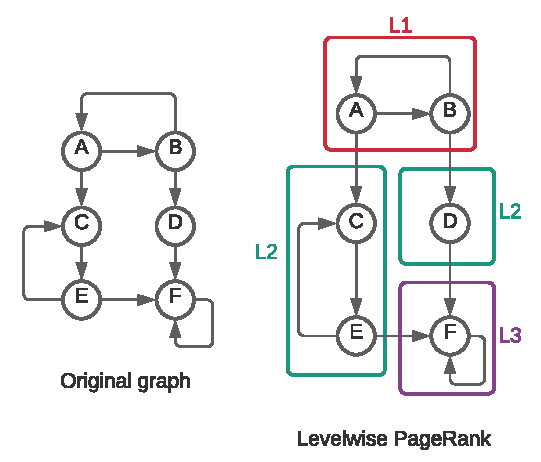
\includegraphics[width=0.48\textwidth]{out/about-levelwise.pdf}
  \caption{Consider a graph with 6 vertices, as shown on the left. This graph has 4 SCCs, C1 with vertices A and B, C2 with vertices C and E, C3 with vertex D, and C4 with vertex F. Its block-graph consists of vertex C1 pointing to C2, which then points to C3. This is the order in which SCCs are processed as per the \levelwisePR{} algorithm.}
  \label{fig:levelwise}
\end{figure}

\begin{algorithm}[!hbtp]
\caption{Algorithm for computing \emph{plain STIC-D PageRank} (static Levelwise) without identical, chain, and dead vertex optimizations. Here, $G$ is the current snapshot of the graph.}
\label{alg:sticd}
\begin{algorithmic}
% \Require{$G$: Graph (V, E)}
\Require{$SCC+TOPO(G)$: finds components of $G$ in topological order grouped by levels in block-graph}
\Function{sticdPR}{$\vars{G}$}
\State $[[C_{11}, C_{12}, \cdots], \cdots] \gets SCC{+}TOPO(G)$
\ForAll{$u \in V$}
  \State $pr_u = 1/n$
\EndFor
\ForAll{$i \in range(0, levels)$}
  \ForAll{$C_{ij} \in [C_{i1}, C_{i2}, \cdots]$} \textbf{in parallel}
    \State $pr \gets \textsc{calculateRanks}(G, [C_{ij}], pr)$ \\ \Comment{see Algorithm \ref{alg:static}}
  \EndFor
\EndFor
\Return{$pr$}
\EndFunction
\end{algorithmic}
\end{algorithm}





\subsection{nvGraph PageRank}

The NVIDIA Graph Analytics library (nvGraph)~\cite{pr-nvgraph} is a library of high performance parallel graph algorithms. It has been designed keeping the core functionality of all graph operations centered around sparse linear algebra. The library provides graph construction and manipulation primitives that are optimized for NVIDIA GPUs. It also provides optimized implementations for the core computation of sparse matrix vector products using a semi-ring model, with automatic load balancing for any sparse pattern. The library is currently distributed as a part of the larger RAPIDS framework and contains implementations for a wide range of traditional graph processing algorithms like community detection, shortest paths, link analysis, connected components, and flow. It has support for three different graph storage formats: Compressed Sparse Row (CSR), Compressed Sparse Column (CSC), and the Coordinate list (COO). The library also allows a program to extract a subgraph based on the list of vertices or list of edges. 




%\textbf{Spider traps} are groups of vertices (or even just a single vertex) which \emph{only out-link each other}. Eventually, spider traps absorb all the \emph{importance} and such vertices delay or hamper the PageRank calculation. A solution to this issue is to use a \emph{damping factor $\alpha$} (also called \emph{taxation}), which controls the probability with which the surfer follows one of the links on a given page \cite{pr-kang}. It is usually set to \emph{0.85}. Which means there is a \emph{15\% chance} of the surfer teleporting to a random page at any time.
%On the other hand, \textbf{dead ends} (or \emph{dangling vertices}) are vertices which have \emph{no out-links}. This means the random-surfer has \emph{nowhere} to go. In the presence of such web pages (vertices), the \emph{probability transition matrix} is not \emph{column stochastic}, which is a \emph{requirement} for \kk{PageRanks to converge.} Several authors suggest different ways to handle this scenario, including  teleport  \cite{pr-deeper01,pr-kang},  adding self loops to such vertices or all vertices, or removing all dead ends recursively. The PageRanks obtained do differ based on the strategy employed to deal with dead ends.
% \emph{Markov chains}. This can cause \emph{importance} to \emph{leak out} of the graph. The most commonly used solution to this is to allow the surfer to \emph{always} \textbf{teleport} to a random page upon reaching a \emph{dead end} \cite{pr-deeper01, pr-kang}. This however, is \emph{not} an ideal strategy for handling dead ends with \emph{dynamic PageRank} since any \emph{affected dead end (including dead ends in the previous snapshot)} can affect the ranks of \emph{all vertices} in the graph. Note that, \emph{affected vertices} are those which are either \emph{changed vertices}, or are \emph{reachable} from changed vertices. \emph{Changed vertices} are those which have an edge added or removed between it and another (changed) vertex.
%Other possible strategies of \textbf{handling dead ends} include \emph{adding self loops to dead ends} (used here), \emph{adding self loops to all vertices}, or even \emph{removing all dead ends recursively} (as removing existing dead ends can introduce new dead ends). None of these require a \emph{common teleport contribution} calculation per iteration, or enable a single affected vertex to affect ranks of all vertices (unlike \emph{teleport} strategy). It important to note however that \emph{ranks} obtained with the use of each such dead-end handling strategies can be \emph{significantly} different, because of their semantic difference.


% A \emph{block-graph} is then obtained, where each \emph{vertex} in the \emph{block-graph} denotes an \emph{SCC} in the \emph{original graph}, and the \emph{edges} represent \emph{cross-edges between SCCs}.  


%\kk{Move this to Preliminaries. Talking about Levelwise/Monolithic at this stage is premature. \textbf{Levelwise PageRank} is one such technique for the PageRank algorithm. It decomposes the input graph into a directed acyclic block-graph of strongly connected components, and processes them in topological order, one level at a time \cite{pr-sticd16}. It enables one to perform PageRank computation in a \textit{distributed fashion} \textbf{without per-iteration communication}. In contrast, the standard method of PageRank computation requires all vertices in the graph to be processed in each iteration, and performing it in a distributed manner would require communicating ranks of vertices between processors in every iteration. It should however be noted that this technique can \textit{only} be applied on graphs \textit{without dead ends} (discussed in detail later).}
%\su{Ok sir but i was thinking of explaining the motivation of the paper right in the first paragraph.}
% (vertices with no outgoing edges, also commonly called dangling vertices). This is discussed in detail later. However, this is usually a non-issue as they can be dealt with by adding self-loops to such vertices. Other possible alternatives include adding self-loops to all the vertices, or even removing all dead ends recursively (as removing existing dead ends can introduce new dead ends). It is also important to note that ranks obtained with the use of each such dead-end handling strategies can be significantly different, because of the semantic difference between each strategy.


% \kk{Subhajit: The discussion on monolithic and levelwise will go to the next section on algorithmic details.}
% \su{Sir, i wrote about monolithic and levelwise in preliminaries to include details already known before this paper. Such as for monolithic is discuss the standard approach for computing PageRank where all vertices are processed. Similarly with levelwise is write about the algorithm published by paritosh in 2016. In the algorithmic approaches section i only then include new modifications to each algorithm.}


\section{Algorithmic approaches}
Let $G$ be the previous snapshot of the graph, and $B$ be the set of edges (graph delta/batch) that are to be inserted/deleted. If the batch of edges $B$ consists of edges to be inserted then the new graph $G' := G \cup B$, whereas if $B$ consists of edges to be deleted, then the new graph $G' = G \setminus B$. We use $pr_v$ to denote the PageRank of a vertex $v$, $in_v := \{u \mid (u, v) \in E\}$ to denote the set of incoming neighbors of $v$,  $indeg_v = |in_v|$ to denote the in-degree of $v$. Similarly, $out_v$ and $outdeg_v$ correspond to the out-neighbors and out-degree of $v$. Finally, $n$ is the total number of vertices in the graph. We assume that the SCCs of $G'$ and those of $G$ are identical. This is a common assumption made in other papers dealing with dynamic centrality measures \cite{cent-shukla20,jamour,cc-mccoll13,ipdps22}.

We say that a vertex $v$ is affected due to the insertion/deletion of a batch of edges if the PageRank of $v$ in $G'$ differs from the PageRank of $v$ in $G$. The main idea behind our algorithms is to identify affected vertices as follows. Let $C$ be an SCC of $G'$. If $C$ or an ancestor of $C$ in the topological order of the SCCs of $G'$ have an edge from $B$, then we say that all vertices in $C$ are affected.
% If an SCC $C$ has an affected vertex, then the SCC $C$ is said to be an affected component.

In this section, we describe the two algorithms we propose to obtain the PageRank of vertices in a graph on addition/deletion of a batch of edges. One feature of both of these algorithms is that they (re)compute the PageRank of only vertices that are affected by the insertion/deletion of edges.




\subsection{Dynamic Monolithic PageRank}

Let $G'_{SCC}$ be the block-graph of $G'$. We first identify all the affected SCCs of $G'$, and recompute the PageRank of vertices in the set of SCCs $S := \{C \mid $ \mbox{$C$ is an affected SCC of $G'$} \}. Initial ranks of the vertices are computed from the ranks of vertices in the previous graph snapshot using Algorithm \ref{alg:adjust-ranks}. PageRank computation is then performed on all affected SCCs in each iteration, until ranks of all affected vertices converge (based on given tolerance). The algorithm for \monolithicPR{} is shown in Algorithm \ref{alg:monolithic}. In Algorithm~\ref{alg:monolithic}, $MIN\_WORK$ is the minimum number of vertices that are processed together for computing PR in a monolithic manner. We also partition the vertices based on an in-degree based threshold to efficiently allocate threads for each vertex. This threshold is controlled by $SWITCH\_DEG$, below which we partition so as to allocate one thread per vertex and if above, we allocate one block of threads to each vertex.

\begin{algorithm}[!hbtp]
\caption{Calculation of initial ranks for \emph{dynamic PageRank}, given ranks of vertices for \emph{previous snapshot} of the graph $F(V,E)$, and the \emph{current} graph $G(V,E)$.}
\label{alg:adjust-ranks}
\begin{algorithmic}
% \Require{$F$: Previous snapshot of the graph}
% \Require{$G$: Current snapshot of the graph}
% \Require{$prev$: Ranks of vertices in $F$}
\Function{adjustRanks}{$\vars{F}, \vars{G}, \vars{prev}$}
\State $old \gets F.vertices() \cap G.vertices()$
\State $new \gets G.vertices() - F.vertices()$
\Return{$old: prev[old] \times |V(F)|/|V(G)|, new: 1/|V(G)|$}
\EndFunction
\end{algorithmic}
\end{algorithm}

\begin{algorithm}[!hbtp]
\caption{Algorithm for computing \emph{dynamic Monolithic PageRank}. Here, $F$ is the previous snapshot of the temporal graph, $G$ is the current snapshot, and $prev$ is the initial estimate of ranks (usually it is the \emph{adjusted} previous ranks of vertices).}
\label{alg:monolithic}
\begin{algorithmic}
\Function{dynamicMonolithicPR}{$\vars{F}, \vars{G}, \vars{prev}$}
  \State $MIN\_WORK \gets 10^7$ \Comment{vertices}
  \State $SWITCH\_DEG \gets 64$ \Comment{indegree}
  \State $SCCs \gets affectedSCCs(F, G)$
  \If{$GPU$}
    \State $mergeMiniSCCs(SCCs, G, MIN\_WORK)$
    \State $partitionByIndeg(SCCs, G, SWITCH\_DEG)$
  \EndIf
  \Return $\textsc{monolithicLoop}(G, SCCs, prev)$ \\  \Comment{see Algorithm \ref{alg:static}}
\EndFunction
\end{algorithmic}
\end{algorithm}





\subsection{Dynamic Levelwise PageRank}

\levelwisePR{} differs from the Monolithic approach in the way the affected SCCs are processed. Let $G'_{SCC}$ be the block-graph of $G'$, where $G'$ is the current snapshot of the graph. Initial ranks of the vertices are obtained with the same process as mentioned above. We start by recomputing the PageRanks of vertices in the SCCs grouped by levels $L_i := [C_{i1}, C_{i2}, ...]$ in the block-graph of $G'$ such that $L_i$ is the topmost unprocessed level in $G'_{SCC}$. PageRank computation is then performed on each affected level $L_i$ in sequential order until convergence. This is repeated until all affected SCCs have been processed. The algorithm for \levelwisePR{} is shown in Algorithm \ref{alg:levelwise}.

\begin{algorithm}[!hbtp]
\caption{Algorithm for computing \emph{dynamic Levelwise PageRank}. Here, $F$ is the previous snapshot of the temporal graph, $G$ is the current snapshot, and $prev$ is the initial estimate of pr (usually it is the \emph{adjusted} previous pr of vertices).}
\label{alg:levelwise}
\begin{algorithmic}
\Function{dynamicLevelwisePR}{$\vars{F}, \vars{G}, \vars{prev}$}
  \State $SWITCH\_DEG \gets 64$ \Comment{indegree}
  \State $SCCs \gets affectedSCCs(F, G)$
  \State $mergeByLevel(SCCs, G)$
  \If{$GPU$}
    \State $partitionByIndeg(SCCs, G, SWITCH\_DEG)$
  \EndIf
  \Return{$\textsc{levelwiseLoop}(G, SCCs, prev)$}
\EndFunction

\Statex

\Function{levelwiseLoop}{$\vars{G}, \vars{SCCs}, \vars{prev}$}
  \State $pr \gets prev$
  \ForAll{$SCC \in SCCs$}
    \State $pr \gets \textsc{monolithicLoop}(G, [SCC], pr)$ \\  \Comment{see Algorithm \ref{alg:static}}
  \EndFor
  \Return{$pr$}
\EndFunction
\end{algorithmic}
\end{algorithm}




% Real-world graphs are usually dynamic, with new edges and vertices being inserted or deleted all the time. \emph{Time-evolving ranks} of vertices in such a graph can be obtained by performing a fresh (static) PageRank computation at every snapshot of the graph. Another approach is to use the ranks of vertices in the previous snapshot as \emph{initial ranks} to the algorithm \cite{pr-deeper01}. This approach is called \emph{incremental/dynamic PageRank}. Here however, we consider the two are considered to be somewhat different, i.e., \emph{dynamic PageRank} involves skipping computation on unaffected vertices, while \emph{incremental PageRank} does not.

% With dynamic Levelwise PageRank however, affected components are arranged in topological order of their appearance in the block-graph, . Each component in the block-graph is represented by a vertex, and each cross-edge between two components represents an edge (multiple cross-edges between components are represented by a single edge). A simple example of this process is shown in Figure \ref{fig:levelwise}. Components with with the same level in the block-graph are combined, and each level is processed in sequential order. This is done by performing the entire PageRank computation loop (i.e., multiple iterations) per level until its convergence.
% Like the original algorithm \cite{pr-sticd16}, the input graph is decomposed into a \emph{block-graph} of \emph{SCCs}, and processed in \emph{topological order}, a \emph{level} at a time. Note that each level can be composed of one or more components. \emph{All} the components in a level are processed at the \emph{same time}, \emph{until convergence} (multiple iterations). A level can \emph{only} be processed after its \emph{previous levels} have been \emph{processed} (till convergence). On \emph{GPUs}, in addition to this, vertices in each level are \emph{partitioned by in-degree} similar to \emph{Monolithic} approach, as mentioned above. The formula used for calculating the rank of each vertex is exactly the same as that mentioned for Monolithic PageRank.
% In dynamic mode, the \emph{initial ranks} are obtained from the \emph{previous snapshot} of the graph, and only \emph{affected components} are processed (computation on \emph{unaffected components} is skipped). \emph{Affected components} are obtained by performing a \emph{Depth-First Search (DFS) traversal} of the \emph{block-graph}, from the \emph{changed components}. Algorithm for Levelwise approach is shown in Algorithm \ref{alg:levelwise}.


% \subsection{Dynamic PageRank}
%The \emph{initial} PageRanks are obtained from the \emph{previous snapshot} of the graph, and only \emph{affected vertices} are processed (computation on \emph{unaffected vertices} is skipped).


% \kk{add some pseudo-code that details the steps of the algorithm. Such as: for a batch B of edges added do.}
% \kk{It may be better to write the pseudo-code than the actual code. The pseudo-code will highlight the steps}
% \su{Sir the python-like code is actually pseudo-code!}


% \subsection{Batch Update}
% \subsection{Analysis}


\section{Implementation details}
We start by describing the software implementation of \monolithicPR{} and \levelwisePR{} on the CPU and the GPU. Both algorithms accept the previous and current snapshot of a graph as input, along with the initial ranks of the vertices. SCCs of both graph snapshots are obtained using Kosaraju's algorithm \cite{scc-sharir81} and compared, in order to obtain a list of changed SCCs. From each SCC, depth-first search (DFS) is performed in order to obtain a list of affected SCCs. We use the CSR representation of graphs for PageRank computation in order to have good memory locality. Vertices are reordered as part of preprocessing step, and computed ranks are un-reordered as part of post-processing step.




\subsection{CPU implementation with OpenMP}

With \monolithicPR{}, vertices of affected SCCs are grouped together (as it has been observed to improve performance \cite{gh-levl21}), and selected for PageRank computation, while the remaining vertices are skipped. This is done by arranging the affected vertices (grouped by SCC) at the top of the CSR representation of the graph. The calculation of ranks of affected vertices in each iteration is done is parallel with OpenMP using 32 auto-scheduled threads, such that calculation of ranks of one or more vertices is assigned to each thread.

With \levelwisePR{}, affected SCCs are arranged in a topological order of their appearance in the block-graph. Each SCC in the block-graph is represented by a vertex, and each cross-edge between two SCCs represents an edge (multiple cross-edges between SCCs are represented by a single edge). A simple example of this process is shown in Figure \ref{fig:levelwise}. SCCs in the same level in the block-graph are combined, and each level is processed in sequential order. This is done by performing the entire PageRank computation loop (i.e., multiple iterations) per level until its convergence.




\subsection{GPU implementation}

We discuss the details of how we achieve good device utilization and load balance across threads in our GPU implementation. We first describe the implementation of \monolithicPR{}. As the degree of vertices may be varying widely, we follow the general practice of choosing a thread or block of threads per vertex for calculating ranks. In order to achieve this, vertices in each SCC with an in-degree of $64$ ($SWITCH\_DEG$) or below are considered to be the thread-per-vertex partition where a CUDA kernel assigns the work of calculating the rank for each vertex to a single thread (belonging to a block of $512$ threads). For vertices with in-degree greater than $64$, the CUDA kernel assigns the work of calculating the ranks of each such vertex to a block of threads (consisting of $256$ threads). We observe that grouping vertices by SCCs, and processing each SCC with a thread-per-vertex and a block-per-vertex CUDA kernel after partitioning yields better performance \cite{gh-levl21}. Hence, this is the approach taken here. However as mentioned in \cite{gh-levl21}, small affected SCCs are combined together until they satisfy a minimum work requirement of 10 million vertices ($MIN\_WORK$). We do this in order to reduce the number of kernel calls. Further details of the implementation is given in \cite{gh-levl21}.

The GPU implementation of \levelwisePR{} builds upon the implementation of \monolithicPR{}  in a manner similar to that described in the previous section. 




% Monolithic PageRank (CPU)
% Once calculation of ranks is complete, the error between the ranks of affected vertices in the previous and the current iteration is obtained by computing $L\infty{}-norm$ between the two rank vectors (once again in parallel using 32 auto-scheduled threads, such that the calculation of error of one or more vertices is assigned to each thread with threads cooperating to obtain the final error value). If this error lies below the desired tolerance (usually $10^{-6}$), the main loop terminates. Note that the main loop itself is executed sequentially.

% Levelwise PageRank (GPU)
% Each level thus consists of a number of affected vertices which are processed in parallel with OpenMP using 32 auto-scheduled threads, as mentioned above. Note that the unaffected SCCs of (of any level) are placed at the end of the CSR representation (upon which computation is performed), similar to that of Monolithic PageRank. The main loop completes when each of the levels have sequentially converged.

% Monolithic PageRank (CPU)
% This partitioning of vertices is done by in-degree in order to assist in even work load across blocks of threads in a grid, through the assignment of a thread per vertex to easily process-able vertices with low in-degree, and the assignment of a block per vertex to difficult to process vertices with high in-degree. Note that assigning multiple blocks to a single vertex would require cross-block communication, and thus prove to be counterproductive. It has been observed in \cite{pr-algo21} that grouping vertices by SCCs, and processing each SCC with a thread-per-vertex and a block-per-vertex CUDA kernel after partitioning yields better performance. Hence, this is the approach taken here. However, as mentioned in \cite{pr-algo21}, small affected SCCs are combined together until they satisfy a minimum work requirement of $10 million$ vertices. This is done in order to reduce the number of kernel calls, which can have significant overhead. Further details of the implementation is given in \cite{pr-volta21}.

% Note that the CSR of the vertices are arranged in the order as mentioned above, with the affected SCCs (vertices) being placed at the top of the CSR, and the unaffected vertices being placed at the bottom of the CSR. This again is part of the preprocessing step and is performed on the CPU, where the CSR is generated. This is then copied over to the GPU where the PageRank computation is performed. Once the ranks of vertices have converged, the ranks are copied back from the GPU, and the reordered in original graph order as part of the post-processing step.

% Levelwise PageRank (GPU)
% However, unlike the Algorithm  Monolithic approach, PageRank computation of each level (consisting of one or more affected SCCs) is performed until convergence (i.e., multiple iterations) in a sequential order. The rest of the process, including the preprocessing as well as the post-processing is similar to that of the Monolithic approach.


\section{Results}
We start by describing the details of our experimental platform, the dataset we use, the procedure for generating batches, measuring performance, and then show the results and analysis of our experiments. 



\subsection{Experimental Platform}

For our experiments, we use a system consisting of an NVIDIA Tesla V100 GPU connected to two 48-core CPUs. The Tesla GV100 GPU has 14 TFLOPs of peak single-precision performance, 32 GB/s PCIe bandwidth, and 900 GB/s memory bandwidth. It includes 84 symmetric multiprocessors (SMs), each with 64 independent FP, INT cores, a configurable shared memory size of 96 KB per SM, and is connected to four 4 GB HBM2 DRAM. The Intel Xeon Silver 4116 is a 64-bit, 2.10 GHz (base) Server CPU having 48 x86 cores each, 16.5M L3 cache, and supports DDR4 2400MHz memory. The server is running CentOS 7.9. We use GCC version 9.3 and OpenMP version 5.0 to compile with optimization level 3 (-O3). For all experiments we keep simultaneous multi-threading (SMT) disabled. We use CUDA version 11.3 to compile the GPU programs.
% {\bf CPU:} The system used was a Dell PowerEdge R740 Rack server with two Intel Xeon Silver 4116 CPUs @ 2.10GHz, 128GB DIMM DDR4 Synchronous Registered (Buffered) 2666 MHz (8x16GB) DRAM, 16GB NVIDIA Tesla V100 PCIe GPU (GV100GL), and running CentOS Linux release 7.9.2009 (Core). The Intel Xeon Silver 4116 is a 64-bit, 2.10 GHz (base) Server CPU launched in 2017, that comes with 12 x86 cores each (24 threads with hyper-threading), 16.5M L3 cache, and supports DDR4 2400MHz memory. We use C++ and OpenMP to program our algorithms and the GCC 9 compiler with optimization level 3 (-O3).
% {\bf GPU:} We use an NVIDIA Tesla GV100 (Volta) GPU for our experiments on a GPU. The Tesla GV100 GPU has 14 TFLOPs of peak single-precision performance, 32 GB/s PCIe bandwidth, and 900 GB/s memory bandwidth. It includes 84 SMs, each with 64 independent FP, INT cores, a configurable shared memory size of 96 KB per SM, and is connected to four 4 GB HBM2 DRAM. Volta also supports write-caching (not just load, as previous architectures). Its Address Translation Service (ATS) allows it to access CPU page tables directly (malloc ptr). Its new copy engine does not need pinned memory. Volta's per-thread program-counter, call-stack, allows interleaved executions of warp threads, enabling fine-grained synchronization between threads within a warp. Cooperative groups enable synchronization between warps, grid-wide, multi-GPUs, cross-warp, sub-warp.




\subsection{Dataset}

The graphs we use in our experiments are shown in Table \ref{tab:dataset}. All of them are obtained from the SuiteSparse Matrix Collection \cite{suite19}. For each graph, Table \ref{tab:dataset} lists properties of these graphs including the number of SCCs and the number of levels in the corresponding block-graph. We add self-loops to dead ends in all the graphs. The total number of vertices in the graphs vary from $75$ thousand to $41$  million, and the total number of edges vary from $524$ thousand to $1.1$ billion.

\begin{table}[!hbtp]
\centering
\begin{tabular}{||c||c|c|c|c||}
 \hline
 \textbf{Graph} &
 \textbf{$|V|$} &
 \textbf{$|E|$} &
 \textbf{$SCCs$} &
 \textbf{$Levels$} \\ \hline
 \multicolumn{5}{|c|}{Web Graphs} \\ \hline
  arabic-2005 & 22.7M & 640.0M & 4.0M & 286 \\ \hline
  uk-2005 & 39.5M & 936.4M & 5.8M & 425 \\ \hline
  it-2004 & 41.3M & 1.2B & 6.8M & 278 \\ \hline
  \multicolumn{5}{|c|}{Social Networks} \\ \hline
  soc-Epinions1 & 75.9K & 524.4K & 42.2K & 10 \\ \hline
  soc-LiveJournal1 & 4.8M & 69.5M & 971.2K & 24 \\ \hline
  wiki-Talk & 2.4M & 7.3M & 2.3M & 8 \\ \hline
  \multicolumn{5}{|c|}{Citation/Collaboration Networks} \\ \hline
  cit-Patents & 3.8M & 18.2M & 3.8M & 32 \\ \hline
  coPapersDBLP & 540.5K & 30.5M & 1 & 1 \\ \hline
  amazon-2008 & 735.3K & 5.2M & 90.7K & 6 \\ \hline
  \multicolumn{5}{|c|}{Road/Control-flow Networks} \\ \hline
  italy\_osm & 6.7M & 14.0M & 1 & 1 \\ \hline
  Linux\_call\_graph & 324.1K & 1.3M & 320.1K & 70 \\ \hline
\end{tabular}
\vspace{0.3 cm}
\caption{List of 11 graphs used in our the experiments. Here, $|V|$ is the total number of vertices, $|E|$ is the total number of edges, $SCCs$ is the number of strongly connected components, and $Levels$ is the SCC levels of each fixed graph. The number of vertices and edges are rounded to the nearest thousand (K) or million (M), as appropriate.}
\label{tab:dataset}
\end{table}





\subsection{Batch generation}

We take a base (fixed) graph and generate a batch consisting of random edges to be deleted and inserted. Each batch consists of edge insertions and deletions in an equal mix, and we ensure that no new vertices are added or removed from the graph. The edges to be inserted or deleted are randomly generated, such that edges connecting vertices with high out-degrees have a greater chance of selection. This is done in order to mimic the behaviour of real-world dynamic graphs.
% how performance of each approach is measured, how batches are generated, and then follow up with the details of the specific experiments.

\begin{figure*}[!hbtp]
  \centering

  \subfloat{
    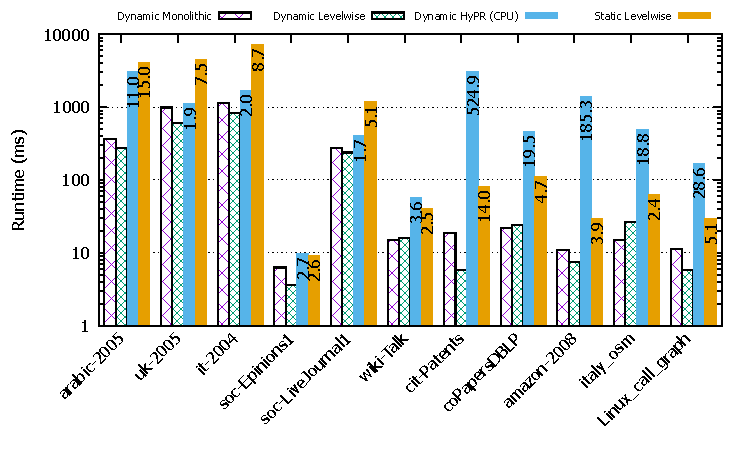
\includegraphics[width=0.48\textwidth]{out/time-omp-am.pdf}
    \label{fig:time-omp-am}
  }
  \subfloat{
    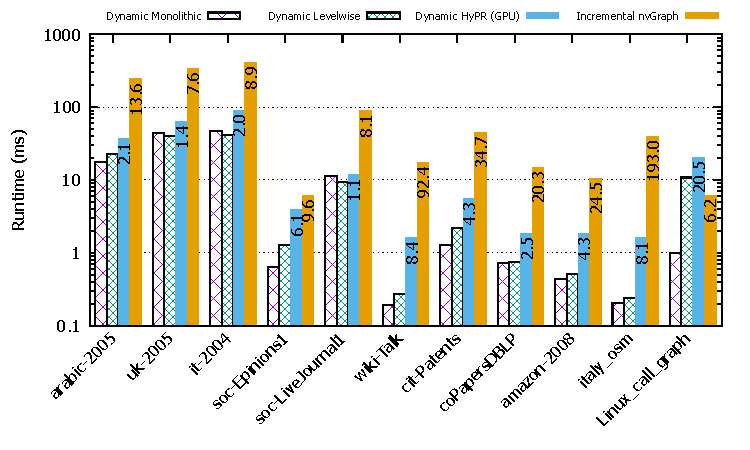
\includegraphics[width=0.48\textwidth]{out/time-cuda-am.pdf}
    \label{fig:time-cuda-am}
  }

  \caption{Time taken for PageRank computation with  \monolithicPR{} and \levelwisePR{} for various batch sizes on the CPU (shown on the left) and the GPU (shown on the right). Batch sizes of 500, 1000, 2000, 5000, and 10000 are used. Time taken with \emph{pure CPU implementation of HyPR} and \emph{plain STIC-D PageRank (static Levelwise)} on the CPU, and speedup of \levelwisePR{} over the two approaches (labeled on top of the respective bars) is also included for comparison. Time taken with \emph{pure GPU implementation of HyPR} and \emph{incremental nvGraph PageRank} on the GPU, and speedup of \monolithicPR{} over the two approaches is included as well.}
  \label{fig:time-am}
\end{figure*}





\subsection{Performance measurement}

We ensure that all the approaches for PageRank computation compared here use the same set of parameters, data types, and other factors determining the time required for computation. We also list out any differences that are beyond our control.

PageRank computation with each approach is performed with a damping factor $d$ of $0.15$, a tolerance $\tau$ of $10^{-6}$, and with a maximum of $500$ iterations. $32-bit$ integers are used for CSR representation, and $32-bit$ floating point values are used for representing ranks for all the approaches. \monolithicPR{} and \levelwisePR{}, along with plain STIC-D PageRank (static Levelwise) use $L\infty{}-norm$ for obtaining the error between the ranks of previous and current iterations. It should however be noted that nvGraph PageRank uses $L2{}-norm$ for error measurement \cite{pr-nvgraph}, which has been observed to converge slower than $L\infty{}-norm$ \cite{gh-levl21}. The measured time in all cases is the rank computation time, and does not include time required to calculate error for convergence check, prepare CSR representation, find affected SCCs, partition vertices by in-degree, group vertices by SCCs, launch kernel (driver overhead), allocate memory, or copy memory between the host (CPU) and the device (GPU). The reported time is the average of multiple runs of respective algorithms. In order to filter out random events affecting the time taken for PageRank computation, each approach is run 5 times and averaged.




\subsection{Results}

\subsubsection{\bf Comparison to Static/Naive Dynamic Approaches}

In this experiment, we compare the performance of \monolithicPR{} (Algorithm \ref{alg:monolithic}) and \levelwisePR{} (Algorithm \ref{alg:levelwise}) with state-of-the-art approaches. In particular, we compare our multicore implementations with the plain STIC-D algorithm (static Levelwise) \cite{pr-sticd16}, which is a static algorithm in the sense that they perform a full recomputation on the new graph. We compare our GPU implementations with the naive dynamic version of nvGraph library implementation of PageRank on a GPU \cite{pr-nvgraph}, a simplified dynamic algorithm which does not skip processing of unaffected vertices (nvGraph does not provide any parameter to control the number of vertices to be processed).
% To the best of our knowledge, there are no dynamic parallel PageRank algorithms to compare our algorithms against. We now describe our experimental results.

\begin{figure*}[!hbtp]
  \centering
  \begin{tikzpicture}
    \draw (0, 0) node[inner sep=0] {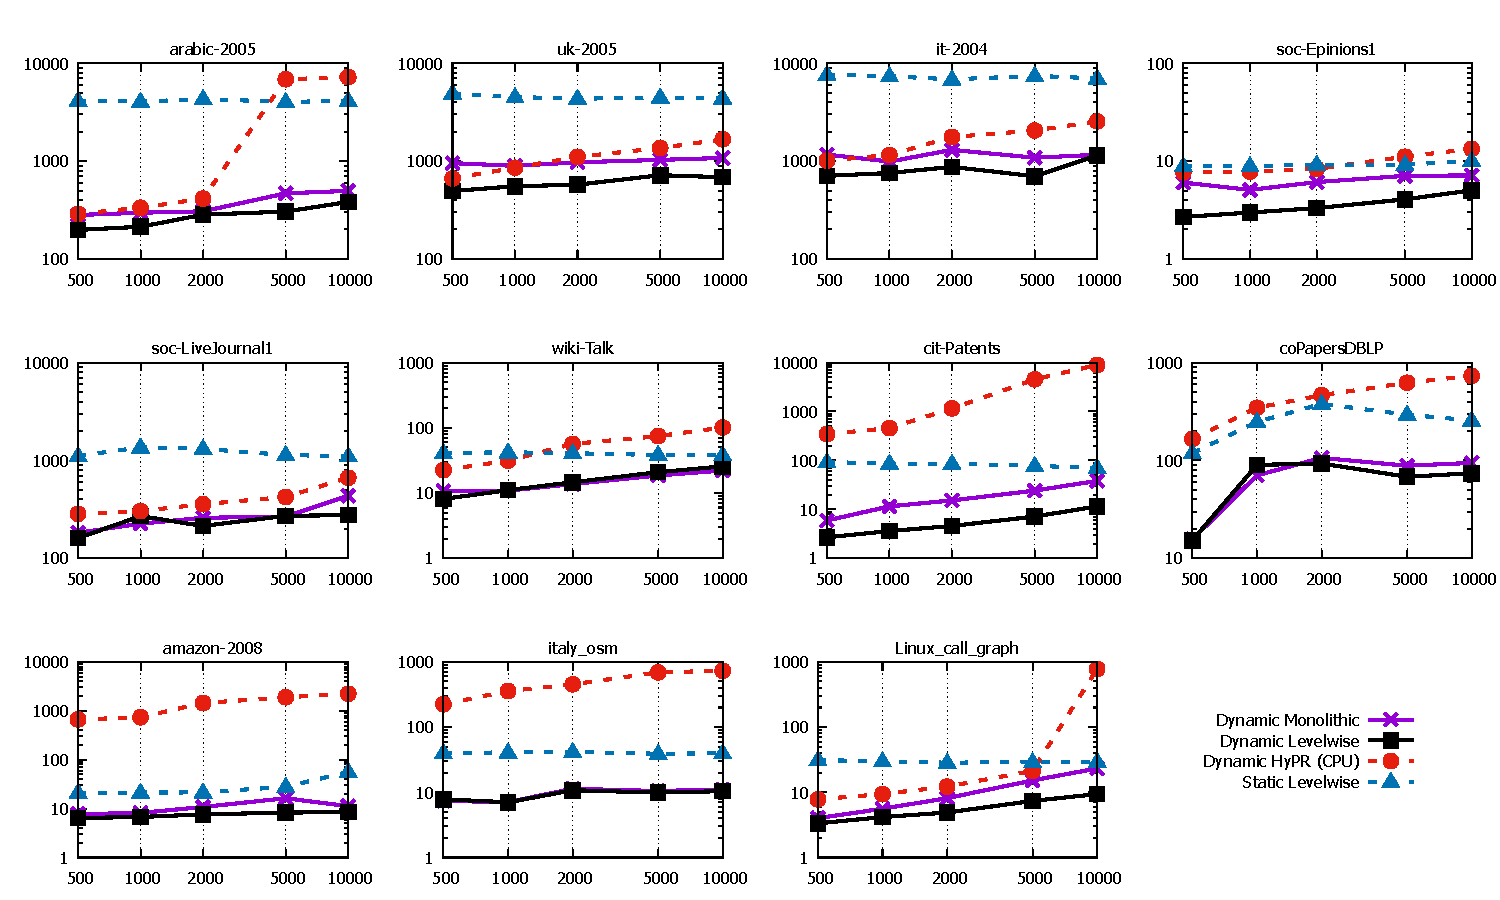
\includegraphics[width=1.00\textwidth]{out/time-omp-all.pdf}};
    \draw (-9.1, 0) node {\rotatebox[origin=t]{90}{Runtime (ms)}};
    \draw (0, -5.7) node {\rotatebox[origin=t]{0}{Batch size}};
  \end{tikzpicture}
  \caption{Time taken for PageRank computation using \monolithicPR{} and \levelwisePR{} on the CPU. Batch sizes of 500, 1000, 2000, 5000, and 10000 are used. Time taken with \emph{pure CPU implementation of HyPR} and \emph{plain STIC-D PageRank (static Levelwise)} is also included for comparison.}
  \label{fig:time-omp-all}
\end{figure*}

\begin{figure*}[!hbtp]
  \centering
  \begin{tikzpicture}
    \draw (0, 0) node[inner sep=0] {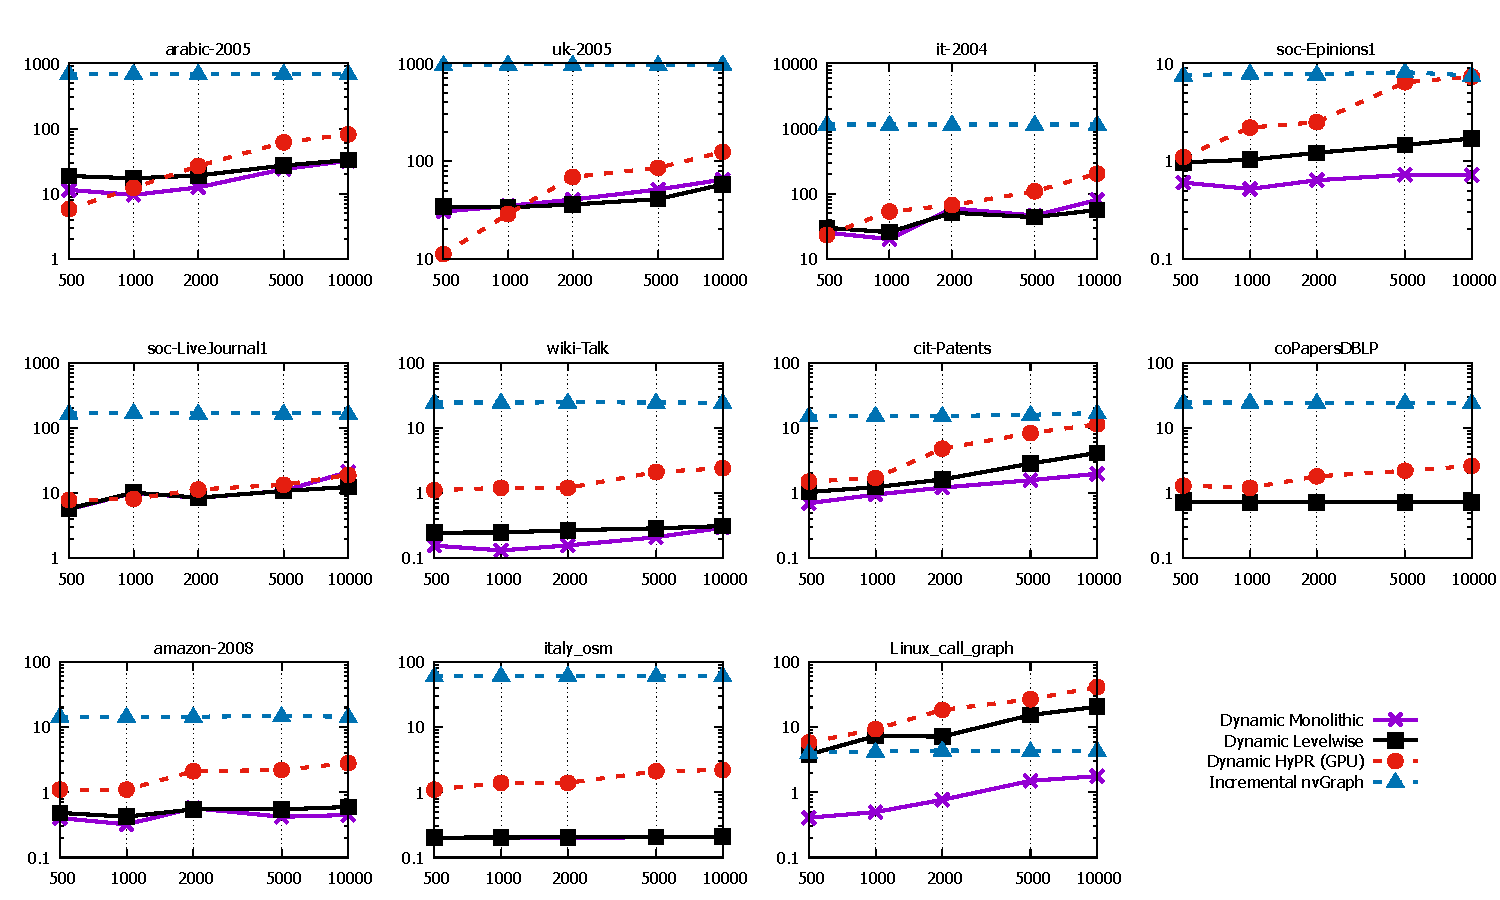
\includegraphics[width=1.00\textwidth]{out/time-cuda-all.pdf}};
    \draw (-9.1, 0) node {\rotatebox[origin=t]{90}{Runtime (ms)}};
    \draw (0, -5.7) node {\rotatebox[origin=t]{0}{Batch size}};
  \end{tikzpicture}
  \caption{Time taken for PageRank computation  using \monolithicPR{} and \levelwisePR{} on the GPU. Batch sizes of 500, 1000, 2000, 5000, and 10000 are used. Time taken with \emph{pure GPU implementation of HyPR} and \emph{incremental nvGraph PageRank} is also included for comparison.}
  \label{fig:time-cuda-all}
\end{figure*}


We experiment with batch sizes of 500, 1000, 2000, 5000, and 10000 edges. The results of this experiment on both the CPU and the GPU is shown in Figure \ref{fig:time-am}. As can be noted from these figures, on the CPU, \monolithicPR{} and \levelwisePR{} achieve an average speedup of 6.1\x and 8.6\x respectively, over the STIC-D algorithm \cite{pr-sticd16}. On the GPU, \monolithicPR{} and \levelwisePR{} achieve an average speedup of 9.8\x and 9.3\x respectively, over the PageRank algorithm from the nvGraph library \cite{pr-nvgraph}. % We observe no significant difference between insertions and deletions and hence the speedup numbers are not reported separately for insertion and deletion batches. 

We observe that \levelwisePR{} performs better on the CPU compared to \monolithicPR{}. \levelwisePR{} is computationally more efficient because it processes SCCs in topological order, avoiding unnecessary recomputation of SCCs that are dependent upon ranks of vertices in other SCCs which have not yet converged. Figure \ref{fig:time-omp-all} shows the detailed run time for each graph and the various batch sizes. We can observe from Figure \ref{fig:time-cuda-all} that \monolithicPR{}{} performs better on the GPU compared to \levelwisePR{}. This is likely due to the presence of levels with insufficient work to keep the GPU busy.

On graphs with a single SCC, viz. {\tt coPapersDBLP} and {\tt italy\_osm} from Table \ref{tab:dataset}, the performance of \levelwisePR{} is almost indistinguishable from \monolithicPR{}. As a single SCC implies a single level in the block graph for \levelwisePR{} to process, its behaviour is identical to that of \monolithicPR{}.




\subsubsection{\bf Comparison to Improved Dynamic approaches}

In this experiment, we compare the performance of the proposed algorithms \monolithicPR{} and \levelwisePR{} with HyPR \cite{hipc19}, a state-of-the-art dynamic PageRank algorithm that only recomputes ranks of affected vertices in the graph. The algorithm from \cite{hipc19} runs in heterogeneous mode and utilizes both the CPU and the GPU simultaneously. To keep our comparison fair, we modify the source code of HyPR to exclusively run either on a CPU or a GPU. We run all the algorithms on a similar set of batches as above.

As seen in Figure \ref{fig:time-am}, we observe a mean speedup of {4.2\x} and {5.8\x} for algorithms \monolithicPR{} and \levelwisePR{} respectively on the CPU, over a pure CPU implementation of HyPR. On the GPU, we observe a mean speedup of {1.9\x} and {1.8\x} for algorithms \monolithicPR{} and \levelwisePR{} respectively, over a pure GPU implementation of HyPR. We also list the detailed run times for each of the approaches with varying batch size on the CPU in Figure \ref{fig:time-omp-all}, and on the GPU in Figure \ref{fig:time-cuda-all}. The speedups can be attributed to grouping of vertices by SCCs and partitioning by in-degree in case of \monolithicPR{}, and due to the processing of affected SCCs in topological ordering in case of \levelwisePR{}.
% of the affected components significantly reduces the amount of work required. This is in contrast to \monolithicPR{} where the work is determined by the affected vertices which incurs significantly higher number of re-computations.
% The performance of HyPR on the GPU seems to approximately proportional to the total number edges, $|E|$. HyPR seems to perform well on web graphs with smaller batch sizes. Why is this? Why it doesn't do th same for larger batch sizes. 
% \kk{this should be comparison to HiPC 2019 paper. The other details are included in the prior subsubsections.}




\subsubsection{\bf Comparison to Single-edge Update}

In this experiment, we study the advantage offered by a batch updates on our algorithms. We take each graph as mentioned in Table \ref{tab:dataset} as the base, and generate a graph delta consisting of a set 10000 edge insertions and deletions, as described in the batch generation section. This graph delta is cumulatively added to the base graph in batches of size 500, 1000, 2000, 5000, and 10000 until the entire graph delta is updated onto the given graph. Each batch, which is a subset of the graph delta, also consists of an equal mix of edge insertions and deletions. After each cumulative update to the graph for the given batch size, PageRank computation is performed with both the dynamic algorithms proposed in this paper, i.e., Algorithms \ref{alg:monolithic} and \ref{alg:levelwise}. Initial ranks are obtained from the ranks of vertices in the previous graph snapshot, as shown in Algorithm \ref{alg:adjust-ranks}. For each approach and batch size combination, the PageRank computation times are measured and summed up. This gives us the total time required for dynamic PageRank computation for a given graph delta, with each approach and batch size combination.

Similar to the process mentioned above, a cumulative single-edge update is performed with the same graph delta upon the base graph, such that edge insertions and deletions alternate with each update. After each update PageRank computation is performed with both the approaches, we obtain the total time needed for the cumulative update by summing up the computation times for each approach. This experiment is performed both on the CPU as well as the GPU.

We observe that a batch update of 5000 edges offers a speedup of {4066\x} and {2998\x} for algorithms \monolithicPR{} and \levelwisePR{} respectively on the CPU, and a speedup of {1712\x} and {2324\x} respectively on the GPU. We show the detailed speedup numbers of  \monolithicPR{} and \levelwisePR{} on each of the 11 input graphs for both the CPU and the GPU in Figure \ref{fig:batch-all}.

From the speedup values, it can be seen that each single-edge update (on average) is only somewhat less expensive than the entire batch update. This seems to suggest that most single-edge updates end up affecting a large number of vertices. This is likely to be the case since batches of edges are generated such that high degree vertices have a higher probability of being changed.

\begin{figure*}[!hbtp]
  \centering

  \subfloat{
    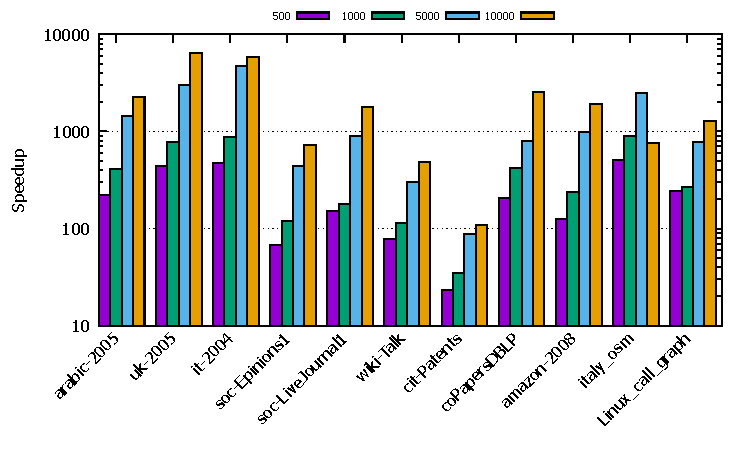
\includegraphics[width=0.48\textwidth]{out/batch-levlomp-all.pdf}
    \label{fig:batch-levlomp-am}
  }
  \subfloat{
    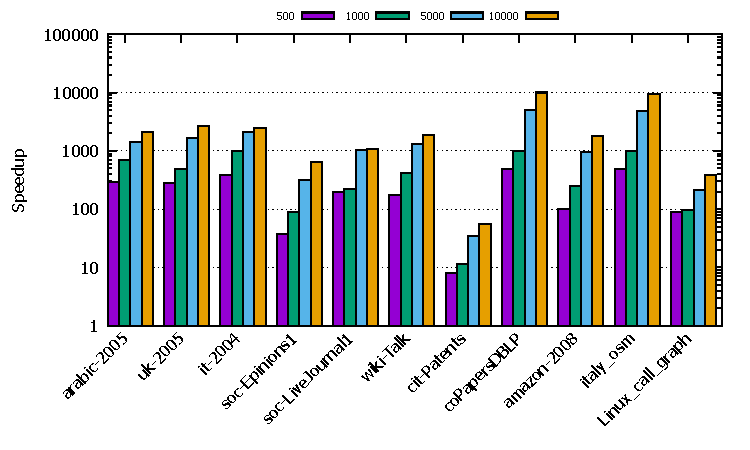
\includegraphics[width=0.48\textwidth]{out/batch-monocuda-all.pdf}
    \label{fig:batch-monocuda-am}
  }

  \caption{Speedup of batched \levelwisePR{} algorithm with respect to cumulative single-edge updates with the same approach on the CPU is shown on the left. Speedup of batched \monolithicPR{} algorithm with respect to cumulative single-edge updates with the same approach on the GPU is shown on the right. Batch sizes of 500, 1000, 5000, and 10000 are shown.}
  \label{fig:batch-all}
\end{figure*}





% \subsection{Batch generation}
% In order to mimic the behaviour of dynamic graphs, a base (fixed) graph is taken and a batch consisting of random edges to be deleted and inserted are generated. Each batch consists of edge insertions and deletions in a 50-50 mix, and it is ensured that no new vertices are added or removed from the graph. The edges to be inserted or deleted are randomly generated, such the edges connecting vertices with high out-degrees have a greater chance of selection.


% To perform our experiments, we do the following preprocessing steps. We first obtain the strongly connected components (SCCs) of the graph using the algorithm of Kosaraju \& Sharir \cite{scc-sharir81}. We sort the SCCs in a topological order of vertices in the block graph, where each SCC represents a vertex and each cross-edge between two SCCs represents  an edge. TODO Multiple cross-edges between SCCs  into a single edge on the block-graph. A simple example of this process is shown in figure \ref{fig:levelwise}. As mentioned before, the vertex order obtained after this process dictates the ordering of  vertices in the CSR representation of the graph. We use this ordering  in our PageRank computation. % Unlike Levelwise PageRank, all vertices (components) were processed in each iteration.
% TODO The convergence criteria for \emph{Monolithic} and \emph{Levelwise PageRank}, \emph{convergence} is reached when the \emph{\textbf{L$\infty$-norm}} between the ranks of \su{\emph{all} vertices (all vertices for monolithic, and vertices in the current level for Levelwise)} in the current and previous iterations falls below the \emph{tolerance value}.
% It is however noted that \emph{nvGraph PageRank} uses \emph{L2-norm} for convergence check \cite{pr-nvgraph-l2norm}, which has been observed to converge \emph{slower} than \emph{L$\infty$-norm} \cite{pr-param21}. \emph{\textbf{nvGraph} PageRank} also seems to use a per iteration \emph{L2-norm rank scaling} (such that sum of square of ranks equals 1) followed by an \emph{L1-norm rank scaling} (such that sum of absolute of ranks equals 1) after the \emph{final iteration}.
% For \emph{dynamic PageRank}, ranks of \emph{affected vertices} are considered for the \emph{L$\infty$-norm}. Ranks of vertices from \emph{previous snapshot} of the graph are \emph{adjusted} before being used as \emph{initial ranks}. It involves a simple \emph{scaling} of ranks based \emph{added/removed vertices}, as shown in Algorithm \ref{alg:adjust-ranks}. A \emph{damping factor} of \emph{0.85}, and a \emph{tolerance} of \emph{$10^{-6}$} is used. The maximum number of iterations allowed is \emph{500}. The PageRank computation is performed on a \emph{Compressed Sparse Row (CSR)} representation of the graph. The \emph{execution time} measured for each test case only includes the time required for \emph{PageRank computation}, including \emph{error calculation}. However, the time required to generate the equivalent graph (if needed), find strongly connected components (SCCs) in topological order (for \emph{Levelwise PageRank}), generate CSR, copy back results from CSR, or allocate memory is \emph{not} included.  With dynamic PageRank, ranks are adjusted from initial ranks.
% \begin{algorithm}[!hbtp]
\caption{Calculation of initial ranks for \emph{dynamic PageRank}, given ranks of vertices for \emph{previous snapshot} of the graph $F(V,E)$, and the \emph{current} graph $G(V,E)$.}
\label{alg:adjust-ranks}
\begin{algorithmic}
% \Require{$F$: Previous snapshot of the graph}
% \Require{$G$: Current snapshot of the graph}
% \Require{$prev$: Ranks of vertices in $F$}
\Function{adjustRanks}{$\vars{F}, \vars{G}, \vars{prev}$}
\State $old \gets F.vertices() \cap G.vertices()$
\State $new \gets G.vertices() - F.vertices()$
\Return{$old: prev[old] \times |V(F)|/|V(G)|, new: 1/|V(G)|$}
\EndFunction
\end{algorithmic}
\end{algorithm}



% \subsection{Performance analysis on CPU}
% \subsection{Performance of Algorithms \ref{alg:monolithic} and \ref{alg:levelwise}}
% In this experiment, we  study the performance of Algorithms [dynamic Monolithic PageRank] and \ref{alg:levelwise}. We compare the performance of our algorithms with state-of-the-art approaches. In particular, we compare our multicore implementation with that of the STIC-D algorithm \cite{pr-sticd16} and with that of the nvGraph library implementation of PageRank on a GPU \cite{pr-nvgraph-l2norm}. Both these algorithms are static algorithms, in the sense that they perform a full recomputation on the new graph. To the best of our knowledge, there are no dynamic parallel PageRank algorithms to compare our algorithms against. We now describe our experimental results.
% In our experiment, we prepare batches of edges to be inserted or deleted from the current graph by choosing such edges uniformly at random. We experiment with batch sizes of  500, 1000, 2000, 5000, and 10000 edges. Each batch of edges fully consists of edges being added or edges being deleted (consists of a 50-50 mix of edges being inserted or deleted, and for single-edge updates, consists only of an edge insertion). 
% REWORD A \emph{single-threaded CPU-based implementation} was used with the first experiment for comparing the approaches, and a \emph{switched thread/block-per-vertex CUDA-based (GPU) implementation} was used with the second one.
%The first experiment used a \textbf{single-threaded CPU-based implementation} to compare the difference in performance of \emph{dynamic Monolithic PageRank}, with \emph{dynamic Levelwise PageRank} on \emph{temporal graphs}. With \emph{(dynamic) Levelwise PageRank}, vertices were grouped by \emph{levels}, which consisted of one or more components in each level. The \emph{level} of each component was obtained from its \emph{topological order} in the \emph{block-graph}. Edges were \emph{inserted} to the graph in \emph{batch sizes} of \emph{500}, \emph{1000}, \emph{5000}, and \emph{10000}. For each batch size, \emph{5 different samples} were taken at different points in time, and their \emph{arithmetic mean (AM)} was obtained.
%Execution time was measured using \emph{std::chrono::high\_performance\_timer}, \emph{5 times} for each test case, and averaged. Statistics of each test case was printed to \emph{standard output (stdout)}, and redirected to a \emph{log file}, which was then processed with a \emph{script} to generate a \emph{CSV file}, with each \emph{row} representing the details of a \emph{single test case}. This \emph{CSV file} was imported into \emph{Google Sheets}, and necessary tables were set up with the help of the \emph{FILTER} function to create the \emph{charts}.


% \kk{Subhajit -- write these as speedup numbers. Not percentages. Speedup = algorithm A time/ algorithm B time, with B being our algorithm and A is the one we are comparing to.}
% \su{Done.}
% \kk{Subhajit: Write one paragraph for CPU and one for GPU. The current plan is to have subsections based on experiments, and not based on platforms. A model is given below.}
% \su{Sir what are the name of subsections?}


% The results of this experiment on the CPU are shown in Figure \ref{fig:time-am} [expt-insert]. As can be seen in these figures, on the CPU Algorithm Levelwise PageRank and Algorithm Monolithic PageRank achieve an average speedup of AAA and BBB respectively, over the STIC-D algorithm \cite{pr-sticd16}. We observe no significant difference between insertions and deletions and hence the speedup numbers are not reported separately for insertion and deletion batches. 
% Figure \ref{fig:time-omp-all} shows the detailed run time for each graph and the various batch sizes. We can observe from Figure \ref{fig:time-cuda-all} that Algorithm Levelwise performs better on the CPU compared to Algorithm Monolithic PageRank. 
% The results of this experiment on the GPU are shown in Figure \ref{fig:time-omp-all} [expt-insert]. As can be seen in these figures, on the GPU Algorithm Levelwise PageRank and Algorithm Monolithic PageRank achieve an average speedup of AAA and BBB respectively, over the PageRank algorithm from the nvGraph library \cite{pr-nvgraph-l2norm}. We observe no significant difference between insertions and deletions and hence the speedup numbers are not reported separately for insertion and deletion batches. 
% Figure \ref{fig:time-omp-all} shows the detailed run time for each graph and the various batch sizes. We can observe from Figure \ref{fig:time-cuda-all} that Algorithm Levelwise performs better on the GPU compared to Algorithm Monolithic PageRank. 


% \kk{Subhajit -- Put these numbers in the earlier paragraphs}


% From the results, it was observed that the speedup of \emph{dynamic Levelwise PageRank} ranges from \emph{0.99x} to \emph{6.25x} for \emph{insertions}, and by \emph{0.99x} to \emph{7.14x} for \emph{deletions}, with respect to \emph{Monolithic} approach (with vertices split by components). For \textbf{edge insertions}, the \textbf{AM speedups} \cite{pr-param21} of \emph{dynamic Levelwise PageRank} are \textbf{2.94x}, \textbf{2.5x}, and \textbf{1.67x} for \emph{batch sizes} of \emph{500}, \emph{1000}, and \emph{10000} respectively. For \textbf{edge deletions}, the \textbf{AM speedups} are \textbf{3.45x}, \textbf{3.03x}, and \textbf{2.22x}. Here, \emph{AM speedup} was obtained by taking the \emph{arithmetic mean (AM)} of time taken for PageRank computation for insertions/deletions of a particular batch size on all graphs, and then obtaining a ratio \emph{relative} to the \emph{Monolithic} approach.


%\su{Sir although figures for only 500, 1000, and 10000 batch sizes, i ran the expt. with $10$ to $10^8$ batch sizes. Single edge update is just too small and in many cases would likely complete in no time. KK: Repeat the single edge update over the entire batch size. In essence, if the bath size is 100, you run 100 single edge updates and then run the 1 batch of 100. What is the time difference between these two?}


% \subsection{Performance analysis on GPU}
% The second experiment is similar to the first experiment, except that it uses a \textbf{switched thread/block-per-vertex CUDA-based (GPU) implementation} \cite{pr-volta21}. Additionally, \emph{nvGraph's incremental PageRank} approach was also included for reference. Note that \emph{nvGraph} does \emph{not} support \emph{dynamic PageRank}. With \emph{(dynamic) Monolithic PageRank}, vertices were grouped by \emph{large components}, and \emph{partitioned by in-degree} based on a suitable \emph{switch-point} \cite{pr-volta21}. \emph{Large components} were obtained by \emph{combining} together components until they satisfied a \emph{min-compute} of $10^7$. With \emph{(dynamic) Levelwise PageRank}, vertices were grouped by \emph{levels}, which consisted of one or more components in each level, and \emph{partitioned by in-degree} similarly. Rest of the process was similar to that of the first experiment.
% From the results of the second experiment it was observed that the speedup of \emph{dynamic Levelwise PageRank} ranges from \emph{1.51x} to \emph{0.02x} for \emph{insertions}, and by \emph{0.63x} to \emph{0.02x} for \emph{deletions}, with respect to \emph{Monolithic} approach (with vertices split by components). For \textbf{edge insertions}, the \textbf{AM speedups} between \emph{dynamic Monolithic} and \emph{Levelwise PageRank} is \textbf{0.13x} for all \emph{batch sizes} of \emph{500}, \emph{1000}, and \emph{10000}. For \textbf{edge deletions}, the \textbf{AM-RATIOs} are \textbf{0.12x}, \textbf{0.12x}, and \textbf{0.18x}.


% \paragraph{Discussion:}
% From the results of the first experiment using a \textbf{single-threaded CPU-based implementation}, it can be inferred that the \emph{Levelwise} approach to PageRank computation, on a \emph{CPU}, is \emph{about 20-30\% faster than} the \emph{Monolithic} approach. This seems intuitive as Levelwise PageRank processes components in \emph{topological order}, and convergence of components on \emph{higher levels} of the block-graph \emph{should ideally} help accelerate the convergence of the \emph{lower levels}. It is also possible that this could be due to \emph{faster satisfaction} of \emph{convergence criterion} of \emph{each level} (with Levelwise approach), in contrast to convergence of \emph{all the vertices} (with Monolithic approach). Analysis of convergence rate of components/levels might help in understanding the cause, which may be explored in future work. Indeed, \emph{slightly higher} error, with respect to nvGraph PageRank, is observed with the \emph{Levelwise approach}. However, given the fact that Levelwise PageRank is a suitable technique for \emph{distributed PageRank computation} for \emph{dead ends free graphs}, it is a small price to pay.
% The second experiment, which uses a \textbf{switched thread / block-per-vertex CUDA-based (GPU) implementation}, suggests that \emph{Levelwise PageRank} is \emph{significantly slower} than \emph{Monolithic PageRank}. This overwhelming increase in PageRank computation time is most likely due to the existence of a large number of \emph{small sized levels}, consisting of small components. This would cause a \emph{large number of CUDA kernel calls} to be made for each level, which can in act as a \emph{major bottleneck} on the system. Thus, the vanilla Levelwise approach would be \emph{unsuitable} for use with \emph{GPU} unless measures are taken to \emph{combine smaller levels/components} in order to ensure sufficient workload on the GPU per kernel call.


% \kk{Are we doing additional optimizations? We should then also add these details to the section on algorithmic details and show the impact of these optimizations. This kind of analysis per graph class and per optimization adds a lot of value to the paper.}
% \su{Sir, ICD optimizations have not been included.}


% \subsubsection{Comparison to Single Edge Update}
% \subsection{Results and Discussion}
% List of experiments : Replicate over CPU, GPU, and multi-GPU
% \begin{itemize}
%   \item Comparison wrt single update
%   \item Comparison wrt nvGraph black box, cuGraph modified as STIC-D
%   \item Batch size Vs Performance
%   \item Scalability? 
% \end{itemize}
% * CPU Vs GPU: Compare across CPU and GPU
% * Versions of STIC-D driven algorithms on various graph classes: which feature is more suitable for which graph class


\section{Conclusion}
We presented two algorithms for dynamic computation of PageRanks in an evolving graph. We observed that \levelwisePR{} algorithm is a suitable approach for CPUs. However on a GPU, smaller levels/components could be combined and processed at a time in order to help improve GPU usage efficiency as \monolithicPR suggests.

We make the following additional observations about our paper. We assumed that the SCCs of the graph do not change due to the batch of updates. If the SCCs change due to the batch of updates, we can apply our algorithms after the obtaining the new SCCs. Further, it is relatively easy to extend our ideas to the case where vertices are inserted/deleted in addition to edges. The links to source code, along with data sheets and charts, for both the experiments \cite{gh-levl21} is included in references.


\small
\bibliographystyle{IEEEtran}
\bibliography{inc/References}
\end{document}
